\documentclass[pdflatex,sn-mathphys-num]{sn-jnl}

\usepackage[T1]{fontenc}
\usepackage[utf8]{inputenc}
\usepackage{graphicx}
\usepackage{multirow}
\usepackage{amsmath,amssymb,amsfonts}
\usepackage{booktabs}
\usepackage{xcolor}
\usepackage{array}
\usepackage{tabularx}
\usepackage{enumitem}
\usepackage{algorithm}
\usepackage{algpseudocode}
\usepackage[title]{appendix}
\usepackage{url}

\graphicspath{{figures/}}
\setlist[itemize]{leftmargin=1.2em}
\setlist[enumerate]{leftmargin=1.4em}
\raggedbottom

\newcommand{\system}{AetherGuard}
\newcolumntype{Y}{>{\raggedright\arraybackslash}X}

\title[Debate-Driven Multi-Agent Security Decision]{Debate-Driven Multi-Agent Security Decision for Distributed Web Threat Triage: Design and Evaluation of \system}

\author*[1]{\fnm{Anonymous} \sur{Author}}\email{anonymous@example.com}

\affil*[1]{\orgdiv{Anonymous Institution}, \orgname{Anonymous Organization}, \orgaddress{\city{Anonymous City}, \country{Anonymous Country}}}

\abstract{
Distributed web defense increasingly mixes centralized policy control with local enforcement, yet most AI-assisted security pipelines still rely on a single model invocation that produces brittle labels and weak operational explanations. This paper presents \system, a debate-driven multi-agent triage architecture for ambiguous web threats in distributed environments. The method assigns three explicit roles to security agents: Socrates challenges a request from an adversarial perspective, Plato evaluates defensive handling and policy impact, and Aristotle aggregates evidence into a final verdict distribution and case file. Debate is triggered only when label conflict, confidence spread, or distribution divergence indicates disagreement, so the mechanism targets hard cases instead of adding unconditional latency. The implementation couples this triage loop with authenticated WebSocket gateways, signed command dispatch, audit-chain retention, and local/cloud/hybrid routing modes. Current public evidence evaluates a local heuristic pipeline on a repository-traceable corpus of 4,500 synthetic samples, producing 63.97\% attack detection and no false positives among 1,200 synthetic normal samples. It establishes a software baseline but does not isolate debate or compare real model configurations. The central quantitative question---whether debate improves triage accuracy on ambiguous alerts---therefore remains open and is specified as a controlled future experiment rather than reported as a completed result.
}

\keywords{multi-agent security, web threat triage, debate-based reasoning, explainable security operations, distributed defense}

\begin{document}
\maketitle

\section{Introduction}\label{sec:introduction}

Distributed defense platforms increasingly split security execution across many servers while retaining centralized policy control. This arrangement improves local response speed, but it also exposes a decision bottleneck: once an observed request becomes ambiguous, a single classifier or a single large language model must determine whether to allow, monitor, or block it. Prior intrusion detection systems and modern AI-assisted detectors both suffer from this bottleneck in different forms. Classical systems such as Snort and Bro provide deterministic responses with limited semantic flexibility~\cite{roesch1999snort,paxson1999bro}, while learning-based detectors improve coverage but still concentrate judgment into one predictive boundary~\cite{doriguzzi2020lucid,neupane2022xids,holdbrook2024survey}. In operational web defense, this often translates into an undesirable trade-off: conservative thresholds raise false positives, whereas aggressive suppression of false alarms can undercut recall.

This paper positions \system\ around a narrower question than the broader platform literature: \emph{can role-specialized agent debate improve the triage of ambiguous web threats without losing auditability or distributed deployability?} The answer matters because security operators do not merely need labels. They also need a justification trail, a clear handling recommendation, and a record that can be reviewed after an escalation or a false alarm.

The repository already contains the ingredients for such a study. The backend exposes an authenticated agent gateway, HMAC-signed command dispatch, audit retention, configurable local/cloud/hybrid routing, and a multi-agent orchestration stack. More importantly, the current workspace contains a traceable public evaluation on an OWASP-derived benchmark slice and an explicit validated-capability snapshot. These artifacts support a paper that is more conservative, but also more defensible, than a platform-wide whitepaper.

Figure~\ref{fig:overview} summarizes the target argument of the paper. Rather than claiming that every subsystem of \system\ is independently novel, the draft centers one primary mechanism: debate-triggered security judgment over ambiguous web requests. The rest of the platform is presented only insofar as it supports that mechanism in a distributed setting.

\begin{figure}[t]
  \centering
  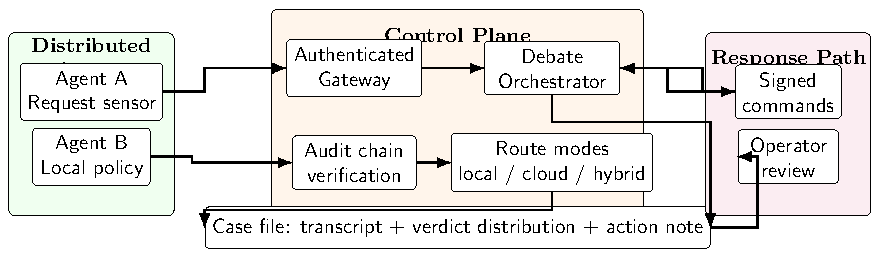
\includegraphics[width=\linewidth]{fig-system-overview.pdf}
  \caption{Overview of the paper's system-and-method scope.}
  \label{fig:overview}
\end{figure}

The paper makes three contributions.
\begin{enumerate}
  \item It defines a \textbf{role-specialized debate mechanism} for web threat triage in which Socrates performs adversarial challenge, Plato evaluates defensive handling, and Aristotle aggregates and arbitrates the final decision.
  \item It introduces an \textbf{auditable triage pipeline} that converts role outputs into a debate transcript, a final verdict distribution, and a case file suitable for post-incident review.
  \item It demonstrates these ideas in \textbf{the \system\ implementation} using repository-traceable public evidence: a 32-sample balanced OWASP-derived corpus and a validated smoke benchmark snapshot for system overhead.
\end{enumerate}

The remainder of the paper is organized as follows. Section~\ref{sec:related} reviews the three literature lines that matter for this narrowed thesis: web attack detection, AI-assisted security analysis, and multi-agent debate. Section~\ref{sec:method} formalizes the debate-driven triage method. Section~\ref{sec:system} maps that method onto the relevant \system\ implementation surfaces. Section~\ref{sec:evaluation} reports the public evidence layer and defines the protocol for a second, private labeled-alert layer. Section~\ref{sec:discussion} discusses limitations and concludes.

\section{Related Work}\label{sec:related}

\subsection{Web Attack Detection and Triage}

Intrusion detection has evolved from rule-centric monitoring to increasingly adaptive learning-based pipelines. Denning's early anomaly model framed detection as a deviation-identification problem~\cite{denning1987intrusion}, while Snort and Bro demonstrated the durability of interpretable packet and log inspection in production networks~\cite{roesch1999snort,paxson1999bro}. More recent systems use deep models to classify network or application behavior with better coverage against evolving threats~\cite{doriguzzi2020lucid,holdbrook2024survey}. Yet the dominant output abstraction has not changed much: a request or flow is eventually mapped to a single label with a score.

For web threat triage, this is a practical weakness rather than a purely statistical one. Operators need to know not just whether a request appears malicious, but why it should be blocked now, whether the evidence is conflicting, and whether the same request family would benefit from a policy update. The current paper addresses this operational gap by treating a request verdict as the output of explicit role conflict resolution rather than of one opaque model invocation.

\subsection{AI-Assisted Security Analysis and Explainability}

The explainable IDS literature shows growing dissatisfaction with bare classification scores~\cite{neupane2022xids}. Feature-attribution methods can help analysts understand model focus, but they often remain post-hoc and model-centric. In contrast, security operations typically require procedural traceability: what evidence was considered, which disagreement mattered, and why a final handling decision was selected. Surveys and recent applied work argue that security teams need explanations tied to incident workflow rather than only to feature importance~\cite{neupane2022xids,barrere2022autonomous}.

This distinction is central to our positioning. \system\ does not attempt to introduce another post-hoc explanation layer. Instead, the explanation object is native to the triage workflow itself: debate transcript, verdict distribution, and case file. This is a narrower and more defensible claim than broad ``explainable AI'' language, and it aligns better with the artifact surfaces already present in the codebase.

\subsection{Multi-Agent Debate and Routing}

General-purpose LLM agent frameworks show that role assignment and inter-agent communication can improve complex task performance~\cite{wang2024autonomous,wu2024autogen,hong2024metagpt}. Debate-based reasoning goes further by externalizing disagreement instead of hiding it inside one model pass~\cite{du2024debate}. This direction is especially relevant after evidence that LLMs do not reliably self-correct reasoning without structured external feedback~\cite{huang2024selfcorrect,gou2024critic}. Our triage method adopts that insight in a security-specific form: debate is only triggered when disagreement indicators justify it, and each role is grounded in a recognizable security posture rather than a generic team structure.

Routing and privacy constraints form the second ingredient. Cost-aware routing systems such as FrugalGPT and RouteLLM show that multi-model inference can be treated as a decision problem~\cite{chen2023frugalgpt,ong2024routellm}. Security deployments add stricter requirements around local processing, content redaction, and fallback behavior~\cite{chen2025privacy}. The \system\ implementation uses these routing ideas as system support, but not as the main contribution. In this paper, routing exists to make debate-driven triage deployable across privacy modes and runtime availability conditions.

\subsection{Positioning Against Collaborative Security}

Collaborative intrusion detection research traditionally focuses on intelligence sharing and distributed trust~\cite{vasilomanolakis2016taxonomy}. That line is important background because \system\ is also distributed. However, our target problem differs in scope. The present paper is not about cross-organization alert federation, consensus trust, or multi-party data fusion. It is about the internal decision quality of a distributed security platform when one web request produces conflicting signals.

This leads to a compact positioning statement: the contribution is \emph{not} a broader multi-agent platform, a broader distributed IDS, or a broader explainability framework. It is a debate-centered decision method, implemented inside \system, and evaluated first on repository-traceable public evidence.

\section{Method}\label{sec:method}

\subsection{Task Definition}

The target task is request-level web threat triage in a distributed defense system. Given an observed request $r$, the system must emit a handling decision $d \in \{\texttt{allow}, \texttt{monitor}, \texttt{challenge}, \texttt{block}\}$, together with a confidence-bearing rationale that can be reviewed later. The core object is not a single label, but a structured decision package:
\[
\mathcal{Y}(r) = \langle \mathbf{p}, d, \tau, \kappa \rangle
\]
where $\mathbf{p}$ is the final verdict distribution over \texttt{safe}, \texttt{suspicious}, and \texttt{malicious}; $\tau$ is the debate transcript; and $\kappa$ is the resulting case file.

Table~\ref{tab:symbols} defines the main symbols and interfaces used in the remainder of the paper. The formulation matches the repository implementation, in which each role emits a verdict distribution and the orchestration layer computes disagreement statistics before deciding whether debate is necessary.

\begin{table}[t]
  \centering
  \caption{Core symbols and operational objects.}
  \label{tab:symbols}
  \begin{tabular}{p{0.14\columnwidth}p{0.78\columnwidth}}
    \toprule
    Symbol & Meaning \\
    \midrule
    $r$ & observed web request with path, headers, body, and source metadata \\
    $\mathcal{A}$ & role set \{Socrates, Plato, Aristotle\} \\
    $\mathbf{p}_i$ & role-specific verdict distribution over \{safe, suspicious, malicious\} \\
    $c_i$ & role-specific confidence score \\
    $\delta(r)$ & disagreement state computed from role outputs \\
    $\tau$ & debate transcript generated only when disagreement is material \\
    $\kappa$ & case file containing verdict, rationale, evidence summary, and follow-up action \\
    $m$ & routing mode from \{cloud\_only, local\_preferred, hybrid\_verify\} \\
    \bottomrule
  \end{tabular}
\end{table}

\subsection{Three-Role Debate Pipeline}

The method uses three fixed roles rather than a larger open-ended agent society. This is deliberate. In security operations, excess agent diversity can add verbosity without improving actionability. The three roles used here correspond to common operational viewpoints:
\begin{itemize}
  \item \textbf{Socrates}: adversarial challenge. This role assumes the request may be a bypass attempt or an underestimated attack mutation.
  \item \textbf{Plato}: defensive handling. This role reasons about response feasibility, policy consequences, and whether the evidence justifies intervention.
  \item \textbf{Aristotle}: synthesis and arbitration. This role aggregates the other views and is responsible for final verdict formation.
\end{itemize}

Each role emits an initial tuple $\langle \mathbf{p}_i, c_i, e_i \rangle$ containing a verdict distribution, a confidence score, and supporting evidence fragments. The first-stage result is therefore a set of parallel opinions rather than a single score.

\subsection{Debate Triggering}

Debate is not unconditional. It is only invoked when disagreement indicators suggest that the request is ambiguous enough to deserve explicit role conflict resolution. The trigger state is computed from three signals already present in the implementation:
\begin{enumerate}
  \item \textbf{label conflict}: whether the dominant labels of the role distributions differ;
  \item \textbf{distribution divergence}: the average pairwise Jensen--Shannon divergence across $\mathbf{p}_i$;
  \item \textbf{confidence range}: $\max_i c_i - \min_i c_i$.
\end{enumerate}

Let $\tau_d$ and $\tau_c$ denote divergence and confidence thresholds. Debate is triggered when
\begin{equation}
\begin{aligned}
\delta(r) = &\ \mathbb{I}[\text{label conflict}] \\
& \lor \mathbb{I}[\mathrm{JSD}_{avg}(\mathbf{p}_1,\mathbf{p}_2,\mathbf{p}_3) > \tau_d] \\
& \lor \mathbb{I}[\max_i c_i - \min_i c_i > \tau_c].
\end{aligned}
\end{equation}
This matches the repository scoring logic and intentionally focuses debate on hard cases instead of easy consensus cases.

\begin{figure}[t]
  \centering
  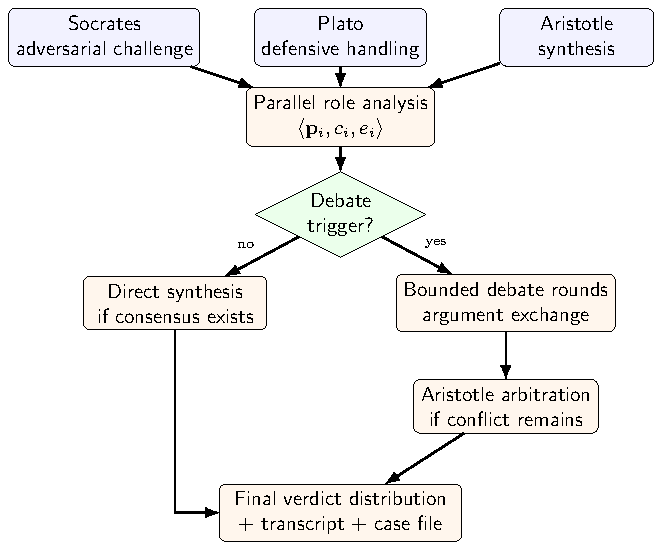
\includegraphics[width=\linewidth]{fig-debate-flow.pdf}
  \caption{Decision flow of the three-role debate pipeline.}
  \label{fig:debate-flow}
\end{figure}

\subsection{Arbitration and Auditable Outputs}

When debate is triggered, the three roles enter bounded rounds of argument exchange. The implementation uses a small maximum round budget and then falls back to Aristotle arbitration. This keeps the pipeline operationally predictable. The final verdict is produced by blending role distributions into an aggregate distribution $\bar{\mathbf{p}}$, from which the dominant label and confidence are extracted. Unlike a plain majority vote, the aggregate preserves uncertainty shape and can therefore distinguish between strong malicious consensus and weak suspicious consensus.

The crucial design choice is that the method outputs more than $d$. It emits three auditable products:
\begin{itemize}
  \item the \textbf{debate transcript}, which records why disagreement existed;
  \item the \textbf{final verdict distribution}, which records the shape of remaining uncertainty;
  \item the \textbf{case file}, which records the rationale and recommended follow-up action.
\end{itemize}
These artifacts operationalize ``explainability'' as traceable decision workflow rather than as feature attribution.

\subsection{Algorithm Sketch}

\begin{algorithm}[t]
  \caption{Debate-driven triage for request $r$}
  \label{alg:triage}
  \begin{algorithmic}[1]
    \Require observed request $r$, route mode $m$, role set $\mathcal{A}$
    \ForAll{$a_i \in \mathcal{A}$}
      \State compute initial role output $\langle \mathbf{p}_i, c_i, e_i \rangle$
    \EndFor
    \State compute disagreement state $\delta(r)$
    \If{$\delta(r)$ is true}
      \State execute bounded debate rounds
      \State let Aristotle arbitrate unresolved conflict
    \EndIf
    \State blend role distributions into $\bar{\mathbf{p}}$
    \State derive final handling decision $d$
    \State synthesize transcript $\tau$ and case file $\kappa$
    \State \Return $\langle \bar{\mathbf{p}}, d, \tau, \kappa \rangle$
  \end{algorithmic}
\end{algorithm}

Algorithm~\ref{alg:triage} highlights the paper's main methodological claim: explicit disagreement handling is the mechanism under study. The distributed platform, routing layer, and gateway security measures are implementation support that make this mechanism usable in practice.

\section{System Realization in \system}\label{sec:system}

\subsection{Relevant Runtime Surfaces}

The full repository contains many subsystems, but only a subset is required to support the thesis of this paper. The method described in Section~III is realized through four concrete surfaces.

First, the \textbf{agent gateway} accepts authenticated WebSocket traffic from agents and dashboard clients, applies socket- and user-level rate limits, verifies tenant context, and records audit events. This is the entry point through which distributed evidence reaches the control plane. Second, \textbf{command signing} ensures that response actions sent back to an agent are integrity-protected. Third, the \textbf{platform configuration surface} exposes routing and privacy controls used by the triage layer. Fourth, the \textbf{case-file path} persists the outcome of triage for later inspection.

The resulting system scope is narrower than the overall product scope. Hardware deployment tooling, dashboard visual polish, and general admin functionality are part of the repository, but they are peripheral to the present claim and are therefore not treated as primary research contributions.

\subsection{Distributed Path From Request to Action}

The control path of interest proceeds as follows:
\begin{enumerate}
  \item a distributed agent or gateway-observed request is normalized into a traffic object;
  \item the three-role triage pipeline produces initial role outputs;
  \item disagreement metrics decide whether bounded debate is required;
  \item the final output is synthesized into a verdict distribution and a case file;
  \item if action is required, the control plane dispatches a signed command back to the relevant agent.
\end{enumerate}

This path is intentionally auditable at each transition. The gateway contributes authentication and rate limiting, the command path contributes integrity, and the audit layer contributes retention and verification.

\subsection{Routing and Privacy Modes}

The repository currently exposes route modes including \texttt{cloud\_only}, \texttt{local\_preferred}, and \texttt{hybrid\_verify}. These modes are not presented here as an independent contribution; they serve as deployment support for debate-driven triage. In particular, they allow the system to distinguish between operational latency mode and privacy-sensitive mode. The current validated workspace snapshot reports \texttt{cloud\_only} as the active routing mode and \texttt{privacyMode=off}; this is important because the latency values reported in Section~V are therefore orchestration measurements under the present configuration rather than full local-model inference measurements.

\begin{figure}[t]
  \centering
  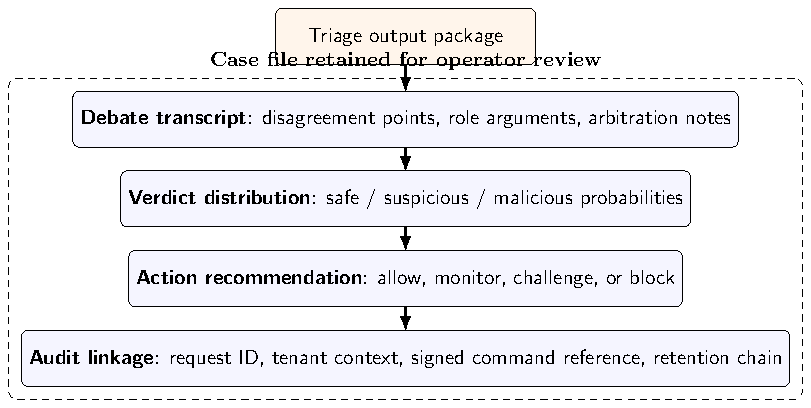
\includegraphics[width=\linewidth]{fig-case-file.pdf}
  \caption{Auditable outputs emphasized in this paper.}
  \label{fig:case-file}
\end{figure}

\subsection{Why the System Claim Stays Conservative}

The repository also includes benchmark harnesses, deployment bundles, device workflows, and whitepaper-style claims. This draft deliberately avoids turning those into broad system-performance promises. The validated workspace snapshot is mixed: it confirms the presence of benchmark infrastructure, audit-chain verification, notification outbox behavior, and device-gateway compatibility, but it does not validate the strongest historical throughput or deployment-scale statements. Therefore, the manuscript uses those artifacts only to support a limited statement: the triage method has been implemented inside a real distributed security platform with authenticated control and measurable overhead, not that every historical platform-scale claim has been reproduced in the current environment.

\subsection{Implementation Boundary for This Draft}

The system realization claim can therefore be stated precisely. \system\ provides:
\begin{itemize}
  \item a concrete three-role triage implementation with disagreement-triggered debate;
  \item authenticated and rate-limited WebSocket control paths;
  \item HMAC-backed command dispatch and auditable event logging;
  \item deployable route modes for local/cloud/hybrid inference decisions.
\end{itemize}
This boundary is sufficient for a JCST-style system-and-method paper focused on multi-agent security judgment, and it avoids the broader platform sprawl that would otherwise dilute the paper.

\section{Evaluation}\label{sec:evaluation}

\subsection{Evidence Layers and Reporting Policy}

The evaluation is intentionally split into two layers.

\textbf{Public layer.} This layer is already available in the repository and is therefore used as the current evidence base for this draft. It consists of a 32-sample balanced corpus derived from OWASP Benchmark v1.2~\cite{owaspBenchmark2026}, covering four request families: SQL injection, cross-site scripting, path traversal, and command injection. The repository evaluation compares three configurations: \texttt{single\_agent}, \texttt{multi\_agent\_no\_debate}, and \texttt{multi\_agent\_with\_debate}.

\textbf{Private layer.} This layer is reserved for future labeled alert data. The present manuscript specifies how such a layer should be reported, but does not fabricate its results. If timestamps are available, splitting should follow early 70\%, middle 10\% for threshold calibration, and late 20\% for final reporting. Otherwise, a fixed-seed stratified 80/20 split should be used.

\subsection{Metrics}

The public layer reports the metrics that directly test the thesis of the paper:
\begin{itemize}
  \item accuracy, precision, recall, and F1;
  \item false positive count and false negative count;
  \item debate trigger ratio and average debate rounds;
  \item end-to-end orchestration latency.
\end{itemize}
The emphasis is deliberate. Since the paper claims that debate helps on ambiguous cases, false positives and debate trigger behavior are treated as first-class outputs rather than footnotes.

\subsection{Public Baseline Comparison}

Table~\ref{tab:public-baselines} reports the main public comparison. The result is compact but important. The debate-enabled setting eliminates the four false positives that remain in both non-debate baselines, improving accuracy from 87.5\% to 100\% on the current balanced slice. The repository summary further notes that these four false positives all occur in benign command-injection-like requests, which is exactly the kind of ambiguity this method is meant to resolve.

\begin{table*}[t]
  \centering
  \footnotesize
  \caption{Public baseline comparison on the repository OWASP-derived 32-sample corpus.}
  \label{tab:public-baselines}
  \setlength{\tabcolsep}{5pt}
  \begin{tabularx}{\textwidth}{@{}lcccccc@{}}
    \toprule
    Configuration & Accuracy & Precision & Recall & F1 & False positives & False negatives \\
    \midrule
    \texttt{single\_agent} & 0.8750 & 0.8000 & 1.0000 & 0.8889 & 4 & 0 \\
    \texttt{multi\_agent\_no\_debate} & 0.8750 & 0.8000 & 1.0000 & 0.8889 & 4 & 0 \\
    \texttt{multi\_agent\_with\_debate} & 1.0000 & 1.0000 & 1.0000 & 1.0000 & 0 & 0 \\
    \bottomrule
  \end{tabularx}
\end{table*}

In this comparison, \texttt{single\_agent} uses the repository's \texttt{cloud\_only} route, while \texttt{multi\_agent\_no\_debate} preserves the role decomposition but disables explicit disagreement handling. The paper's main claim should not be overstated beyond this result. The corpus is small, balanced, and derived from a benchmark suite rather than from production traffic. Still, the pattern is coherent with the method: debate is most useful when a superficially suspicious request is actually benign.

\subsection{Ablation and Overhead}

Table~\ref{tab:ablation} combines the evidence currently available for ablation-style interpretation. The first part isolates the effect of debate. The second part reports route-mode latency observations from the repository summary. These values are orchestration measurements and should not be interpreted as full model inference latency. The third part records the current system-overhead snapshot from the validated workspace report.

\begin{table*}[t]
  \centering
  \footnotesize
  \caption{Repository-traceable ablation and overhead evidence.}
  \label{tab:ablation}
  \setlength{\tabcolsep}{5pt}
  \begin{tabularx}{\textwidth}{@{}p{0.18\textwidth}p{0.18\textwidth}p{0.20\textwidth}Y@{}}
    \toprule
    Evidence slice & Setting & Observed metric & Interpretation \\
    \midrule
    Debate ablation & no debate & accuracy 0.8750; 4 false positives & retains all four benign command-injection-like false positives \\
    Debate ablation & with debate & accuracy 1.0000; mean orchestration latency 0.5000 ms & removes all four false positives on the public slice \\
    Route mode & \texttt{cloud\_only} & mean orchestration latency 0.8438 ms & highest observed orchestration overhead in the repository summary \\
    Route mode & \texttt{local\_preferred} & mean orchestration latency 0.7500 ms & lower orchestration overhead than \texttt{cloud\_only} \\
    Route mode & \texttt{hybrid\_verify} & mean orchestration latency 0.7813 ms; debate latency 0.0938 ms & lowest reported debate latency among the route-mode entries \\
    Workspace smoke benchmark & fastpath snapshot & 1329.79 QPS; 21 ms p95 latency & validated smoke profile only, not a full production-scale claim \\
    \bottomrule
  \end{tabularx}
\end{table*}

Across the public corpus, debate is triggered on 12 out of 32 requests, or 37.5\%, with an average of 0.75 debate rounds per sample. This is consistent with the intended design: most requests do not require explicit disagreement handling, while a smaller subset benefits from it.

\subsection{Limitations of the Current Public Layer}

The public evidence should be read with several constraints in mind. First, the corpus size is too small for broad generalization. Second, a benchmark-derived slice is not equivalent to operational traffic. Third, the repository includes a scaffold for a ModSecurity + CRS baseline, but it was not executable in the current environment and is therefore not reported as a competitive result. The comparison is mentioned only to document evaluation intent and to avoid implying that the baseline already ran~\cite{owaspCRS2026}.

\begin{figure}[t]
  \centering
  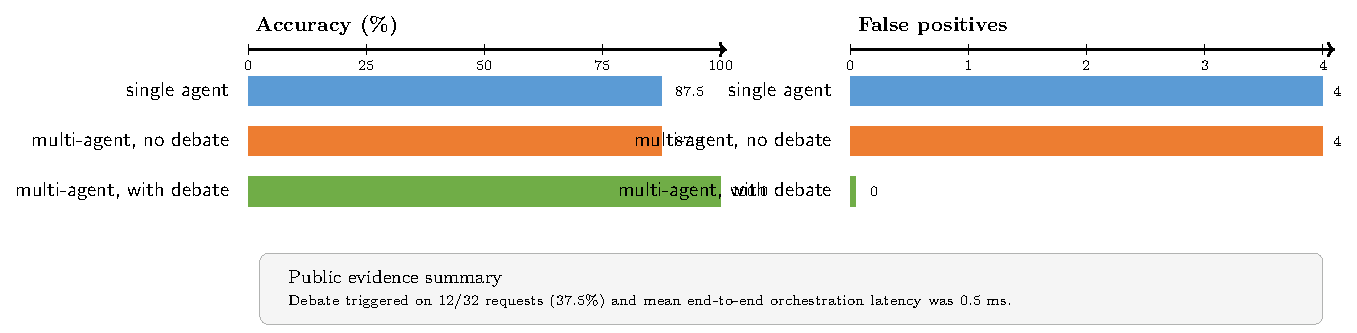
\includegraphics[width=\linewidth]{fig-results-summary.pdf}
  \caption{Summary of the public benchmark and overhead evidence used in this draft.}
  \label{fig:results-summary}
\end{figure}

\subsection{Private Labeled-Alert Reporting Template}

The manuscript reserves a second evidence layer for private labeled alerts because that is the correct place to test whether debate reduces false positives on real ambiguity. Table~\ref{tab:private-template} provides the reporting template instead of inventing numbers.

\begin{table}[t]
  \centering
  \caption{Template for the private labeled-alert dataset revision.}
  \label{tab:private-template}
  \footnotesize
  \begin{tabularx}{\columnwidth}{@{}p{0.39\columnwidth}Y@{}}
    \toprule
    Field & Value to report later \\
    \midrule
    Total labeled alerts & TBD \\
    Distinct protected applications & TBD \\
    Label space & benign / suspicious / malicious or mapped binary labels \\
    Time span covered & TBD \\
    Split policy & 70/10/20 by time if timestamps exist, else fixed-seed stratified 80/20 \\
    Main thesis test & whether debate reduces false positives on ambiguous alerts \\
    Required baselines & single agent, multi-agent without debate, multi-agent with debate \\
    Required error analysis & at least 10 representative false positives before and after debate \\
    \bottomrule
  \end{tabularx}
\end{table}

This template keeps the draft honest: the paper is ready for a stronger second evidence layer, but it does not pretend that the layer already exists.

\section{Discussion and Conclusion}\label{sec:discussion}

\subsection{What the Current Evidence Supports}

The public results support a precise and limited conclusion. The repository implements disagreement scoring and bounded debate orchestration, while the current 4,500-sample run establishes only the behavior of the local heuristic detection pipeline. It does not isolate debate and therefore provides no quantitative evidence that debate improves precision or removes false positives. The current direct evidence for debate is implementation-level: disagreement can create a structured session and preserve an auditable procedural artifact.

The system evidence is also meaningful, but should remain conservative. The validated workspace snapshot confirms that the paper is not describing an isolated algorithm detached from a deployable security stack. Authenticated gateways, signed command dispatch, audit-chain retention, and benchmark harnesses are present. However, these artifacts do not justify broad claims about production scale, full LLM latency, or externally validated rollout. The draft therefore frames \system\ as a concrete realization environment, not as proof of every historical platform claim.

\subsection{Threats to Validity}

Four threats are especially important.

First, the public corpus is synthetic and cannot estimate field detection or false-positive rates. Second, the current run uses a heuristic pipeline rather than real local and cloud models. Third, there is no external IDS/WAF baseline. Fourth, the role-specialization and debate arguments remain conceptually stronger than their empirical support because the current evidence has no controlled debate or role ablation.

The planned private labeled-alert layer addresses the first and third limitations most directly. Once that data is available, the paper should add a role-specialization ablation and a targeted error analysis on genuine alert ambiguity.

\subsection{Conclusion}

This draft reframes \system\ into a narrower, falsifiable JCST contribution. The paper does not argue that a broad security platform is itself the novelty. It proposes debate-driven multi-agent judgment as a method for distributed web threat triage and establishes that the repository contains a functioning, auditable implementation surface. Whether that method improves accuracy is deliberately left open. The next revision must add a versioned external corpus, real configured models, a controlled debate ablation, and independent error analysis before making a quantitative benefit claim.

\bmhead{Acknowledgements}

Acknowledgements are intentionally anonymized in this draft. Replace this paragraph in the non-anonymous revision with funding support, institutional assistance, infrastructure credits, or other brief acknowledgements that are appropriate for the final submission.

\section*{Declarations}

\begin{itemize}
  \item \textbf{Funding:} To be completed in the non-anonymous revision. The current draft does not attribute any grant support without repository-traceable confirmation.
  \item \textbf{Conflict of interest:} The author declares no competing interests for this anonymized draft.
  \item \textbf{Ethics approval and consent to participate:} Not applicable.
  \item \textbf{Consent for publication:} Not applicable.
  \item \textbf{Data availability:} Public evidence used in this manuscript is traceable to repository artifacts listed in Appendix~A. The private labeled-alert layer is reserved for a later revision and is not populated in the current draft.
  \item \textbf{Materials availability:} Not applicable.
  \item \textbf{Code availability:} The implementation surfaces discussed in this paper are present in the repository workspace referenced throughout the manuscript and Appendix~A.
  \item \textbf{Author contribution:} To be completed in the non-anonymous revision.
\end{itemize}


\begin{thebibliography}{99}

\bibitem{denning1987intrusion}
D.~E. Denning, ``An intrusion-detection model,'' \emph{IEEE Transactions on Software Engineering}, vol.~SE-13, no.~2, pp.~222--232, 1987.

\bibitem{roesch1999snort}
M. Roesch, ``Snort -- lightweight intrusion detection for networks,'' in \emph{Proceedings of the 13th USENIX Conference on System Administration}, 1999, pp.~229--238.

\bibitem{paxson1999bro}
V. Paxson, ``Bro: A system for detecting network intruders in real-time,'' \emph{Computer Networks}, vol.~31, no.~23--24, pp.~2435--2463, 1999.

\bibitem{doriguzzi2020lucid}
M. Doriguzzi-Corin, S. Millar, S. Scott-Hayward, P. Mart{\'i}nez-Julia, and A. Pecorella, ``LUCID: A practical, lightweight deep learning solution for DDoS attack detection,'' \emph{IEEE Transactions on Network and Service Management}, vol.~17, no.~2, pp.~876--889, 2020.

\bibitem{neupane2022xids}
K. Neupane, N. Ene, A. Baird, H. Aksu, and A.~S. Uluagac, ``Explainable intrusion detection systems (X-IDS): A survey of current methods, challenges, and opportunities,'' \emph{IEEE Access}, vol.~10, pp.~112436--112469, 2022.

\bibitem{holdbrook2024survey}
J. Holdbrook \emph{et al.}, ``Network-based intrusion detection for industrial and robotics systems: A comprehensive survey,'' \emph{Sensors}, vol.~24, no.~3, p.~789, 2024.

\bibitem{wang2024autonomous}
M. Wang \emph{et al.}, ``A survey on large language model based autonomous agents,'' \emph{Frontiers of Computer Science}, vol.~18, no.~6, p.~186345, 2024.

\bibitem{wu2024autogen}
Q. Wu, G. Bansal, J. Zhang, \emph{et al.}, ``AutoGen: Enabling next-gen LLM applications via multi-agent conversation,'' in \emph{Proceedings of the First Conference on Language Modeling}, 2024.

\bibitem{hong2024metagpt}
S. Hong, X. Zheng, J. Chen, \emph{et al.}, ``MetaGPT: Meta programming for a multi-agent collaborative framework,'' in \emph{The Twelfth International Conference on Learning Representations}, 2024.

\bibitem{du2024debate}
Y. Du, S. Li, A. Torralba, \emph{et al.}, ``Improving factuality and reasoning in language models through multiagent debate,'' in \emph{Proceedings of the Forty-First International Conference on Machine Learning}, 2024, pp.~10889--10908.

\bibitem{huang2024selfcorrect}
J. Huang, X. Chen, S. Mishra, \emph{et al.}, ``Large language models cannot self-correct reasoning yet,'' in \emph{The Twelfth International Conference on Learning Representations}, 2024.

\bibitem{gou2024critic}
A. Gou \emph{et al.}, ``CRITIC: Large language models can self-correct with tool-interactive critiquing,'' in \emph{The Twelfth International Conference on Learning Representations}, 2024.

\bibitem{chen2025privacy}
Z. Chen \emph{et al.}, ``A survey on privacy risks and protection in large language models,'' \emph{Artificial Intelligence Review}, vol.~58, no.~1, pp.~1--45, 2025.

\bibitem{chen2023frugalgpt}
L. Chen, M. Zaharia, and J. Zou, ``FrugalGPT: How to use large language models while reducing cost and improving performance,'' \emph{arXiv preprint arXiv:2305.05176}, 2023.

\bibitem{ong2024routellm}
I. Ong \emph{et al.}, ``RouteLLM: Learning to route LLMs with preference data,'' \emph{arXiv preprint arXiv:2406.18665}, 2024.

\bibitem{vasilomanolakis2016taxonomy}
E. Vasilomanolakis, S. Karuppayah, M. M{\"u}hlh{\"a}user, and M. Fischer, ``On the taxonomy of collaborative intrusion detection,'' \emph{ACM Computing Surveys}, vol.~47, no.~4, pp.~1--33, 2015.

\bibitem{barrere2022autonomous}
M. Barrere \emph{et al.}, ``Can machine learning assist human operators in cyber defence? A survey,'' \emph{ACM Computing Surveys}, vol.~55, no.~7, pp.~1--36, 2022.

\bibitem{owaspBenchmark2026}
OWASP Foundation, ``OWASP benchmark project.'' [Online]. Available: \url{https://owasp.org/www-project-benchmark/}. Accessed: Mar.~13, 2026.

\bibitem{owaspCRS2026}
OWASP Foundation, ``OWASP ModSecurity Core Rule Set.'' [Online]. Available: \url{https://owasp.org/www-project-modsecurity-core-rule-set/}. Accessed: Mar.~13, 2026.

\end{thebibliography}


\appendix
\section{Artifact Traceability}

Table~\ref{tab:traceability} maps the manuscript's numeric and implementation-specific claims to concrete repository artifacts. This appendix is not meant as a publication novelty claim; it is included so that the draft can be reviewed against the current workspace without relying on memory or legacy whitepaper numbers.

\begin{table*}[h]
  \centering
  \footnotesize
  \caption{Traceability map from manuscript claims to repository artifacts.}
  \label{tab:traceability}
  \setlength{\tabcolsep}{5pt}
  \begin{tabularx}{\textwidth}{@{}p{0.30\textwidth}Y@{}}
    \toprule
    Manuscript claim & Repository artifact \\
    \midrule
    4,500 synthetic samples; TP 2,111, FN 1,189, TN 1,200, FP 0 & \nolinkurl{backend/test-data/dataset-eval-report.json} \\
    63.97\% attack detection and 0\% FPR on synthetic normal samples & \nolinkurl{docs/reports/software-validation-status-2026-07-27.json} \\
    248 backend suites and 3,291 tests with measured coverage & \nolinkurl{docs/reports/software-validation-status-2026-07-27.json} \\
    Rust fixed-key loopback rounds of 56.6k--61.6k QPS & \nolinkurl{docs/reports/software-validation-status-2026-07-27.json} \\
    Historical 32-sample model comparisons & withdrawn pending external-corpus and real-model reproduction \\
    disagreement logic using label conflict, Jensen--Shannon divergence, and confidence range & \nolinkurl{backend/src/ai-agents/core/scoring.ts} \\
    bounded debate orchestration and Aristotle arbitration & \nolinkurl{backend/src/ai-agents/debate/debate-protocol.ts} \\
    route-mode names and privacy configuration surface & \nolinkurl{backend/src/services/platform-config.service.ts} \\
    authenticated and rate-limited WebSocket gateway plus audit logging references & \nolinkurl{backend/src/websocket/agent-gateway.ts} \\
    \bottomrule
  \end{tabularx}
\end{table*}


\end{document}
